% =============================================================================
% COPYRIGHT AND DISCLAIMER
% =============================================================================
% This file is provided as a convenience template for competition participants.
% By using it, you accept full responsibility for compliance with all applicable
% copyright, licensing, and usage rules of the Association for Computing
% Machinery (ACM) and of any LaTeX packages you load (including, without
% limitation, the "acmart" document class and related ACM materials).
%
% Consult ACM's official publication, template, and copyright policies before
% using this setup for any purpose other than this competition. Do not assume
% that this template may be reused, redistributed, or submitted elsewhere
% without independently verifying ACM's current rules.
%
% Use of the "acmart" class, the "sigconf" option, or ACM-style formatting in
% this template does NOT mean that this report, this competition, its organizers,
% or any resulting PDF is sponsored, endorsed, affiliated with, or published by
% ACM. ACM trademarks and branding remain the property of ACM.
%
% Template packages live in preamble.tex.
% Citations live in main.bib. Edit this file with your paper content.
% =============================================================================

\documentclass[sigconf]{acmart}
% =============================================================================
% Template setup — participants normally do not edit this file.
% Author content belongs in main.tex; citations belong in main.bib.
% \documentclass lives in main.tex so Overleaf does not treat this file as root.
% =============================================================================

% --- Competition / non-ACM-submission friendly rights metadata -------------
\setcopyright{none}
\settopmatter{printacmref=false}
\acmConference[Kaggle Competition]{Filament Segmentation Challenge}{2026}{\href{https://www.kaggle.com/competitions/filament-segmentation-2026}{kaggle.com/competitions/filament-segmentation-2026}}
\acmBooktitle{Competition Report}
\acmDOI{}
\acmISBN{}

% --- Author guidance text --------------------------------------------------
% \guide{...} is gray italic while \guideStyletrue; omitted from the PDF if false.
% Flip the switch in main.tex after % =============================================================================
% Template setup — participants normally do not edit this file.
% Author content belongs in main.tex; citations belong in main.bib.
% \documentclass lives in main.tex so Overleaf does not treat this file as root.
% =============================================================================

% --- Competition / non-ACM-submission friendly rights metadata -------------
\setcopyright{none}
\settopmatter{printacmref=false}
\acmConference[Kaggle Competition]{Filament Segmentation Challenge}{2026}{\href{https://www.kaggle.com/competitions/filament-segmentation-2026}{kaggle.com/competitions/filament-segmentation-2026}}
\acmBooktitle{Competition Report}
\acmDOI{}
\acmISBN{}

% --- Author guidance text --------------------------------------------------
% \guide{...} is gray italic while \guideStyletrue; omitted from the PDF if false.
% Flip the switch in main.tex after % =============================================================================
% Template setup — participants normally do not edit this file.
% Author content belongs in main.tex; citations belong in main.bib.
% \documentclass lives in main.tex so Overleaf does not treat this file as root.
% =============================================================================

% --- Competition / non-ACM-submission friendly rights metadata -------------
\setcopyright{none}
\settopmatter{printacmref=false}
\acmConference[Kaggle Competition]{Filament Segmentation Challenge}{2026}{\href{https://www.kaggle.com/competitions/filament-segmentation-2026}{kaggle.com/competitions/filament-segmentation-2026}}
\acmBooktitle{Competition Report}
\acmDOI{}
\acmISBN{}

% --- Author guidance text --------------------------------------------------
% \guide{...} is gray italic while \guideStyletrue; omitted from the PDF if false.
% Flip the switch in main.tex after \input{preamble}.
%
% Do not use \guide{...} for \email{...}.
\usepackage{xcolor}
\newif\ifguideStyle
\guideStyletrue
\newcommand{\guide}[1]{%
  \ifguideStyle
    {\color{gray!65}\itshape #1}%
  \fi
}

% --- Math ------------------------------------------------------------------
% Do NOT load amssymb (or amsfonts): acmart already loads newtxmath, which
% defines the same symbols (e.g. \Bbbk) and causes a conflict on Overleaf.
% amsmath is already provided by acmart; mathtools extends it.
\usepackage{mathtools}

% --- Figures ---------------------------------------------------------------
% graphicx is already loaded by acmart
\usepackage{subcaption}

% --- Tables ----------------------------------------------------------------
% booktabs is already loaded by acmart
\usepackage{tabularx}
\usepackage{multirow}

% --- Bibliography style is set in main.tex (ACM-Reference-Format) ----------
.
%
% Do not use \guide{...} for \email{...}.
\usepackage{xcolor}
\newif\ifguideStyle
\guideStyletrue
\newcommand{\guide}[1]{%
  \ifguideStyle
    {\color{gray!65}\itshape #1}%
  \fi
}

% --- Math ------------------------------------------------------------------
% Do NOT load amssymb (or amsfonts): acmart already loads newtxmath, which
% defines the same symbols (e.g. \Bbbk) and causes a conflict on Overleaf.
% amsmath is already provided by acmart; mathtools extends it.
\usepackage{mathtools}

% --- Figures ---------------------------------------------------------------
% graphicx is already loaded by acmart
\usepackage{subcaption}

% --- Tables ----------------------------------------------------------------
% booktabs is already loaded by acmart
\usepackage{tabularx}
\usepackage{multirow}

% --- Bibliography style is set in main.tex (ACM-Reference-Format) ----------
.
%
% Do not use \guide{...} for \email{...}.
\usepackage{xcolor}
\newif\ifguideStyle
\guideStyletrue
\newcommand{\guide}[1]{%
  \ifguideStyle
    {\color{gray!65}\itshape #1}%
  \fi
}

% --- Math ------------------------------------------------------------------
% Do NOT load amssymb (or amsfonts): acmart already loads newtxmath, which
% defines the same symbols (e.g. \Bbbk) and causes a conflict on Overleaf.
% amsmath is already provided by acmart; mathtools extends it.
\usepackage{mathtools}

% --- Figures ---------------------------------------------------------------
% graphicx is already loaded by acmart
\usepackage{subcaption}

% --- Tables ----------------------------------------------------------------
% booktabs is already loaded by acmart
\usepackage{tabularx}
\usepackage{multirow}

% --- Bibliography style is set in main.tex (ACM-Reference-Format) ----------

\newcommand{\pqAll}{0.450}
\newcommand{\pqAllLow}{0.440}
\newcommand{\pqAllHigh}{0.460}
\newcommand{\sqAll}{0.68}
\newcommand{\pqHuman}{0.344}
\newcommand{\thirdOne}{0.34}
\newcommand{\thirdTwo}{0.33}
\newcommand{\thirdMethod}{0.44}
\newcommand{\thirdFrames}{114}
\newcommand{\dqHuman}{0.54}
\newcommand{\sqHuman}{0.63}
\newcommand{\pqPublic}{0.39}
\newcommand{\inferenceMinutes}{60}
\newcommand{\inferenceGpu}{one Tesla T4}
\newcommand{\pqOracle}{0.54}
\newcommand{\tauChosen}{0.24}
\newcommand{\nFrames}{707}
\newcommand{\nViews}{1\,154}
\newcommand{\nDrawings}{8\,199}
\newcommand{\nMulti}{296}
\newcommand{\nFeatures}{33}
\newcommand{\detectorList}{a YOLO11m-seg at $1536^2$ pixels (80 epochs) and a YOLO11s-seg at $1280^2$ pixels (60 epochs)}
\newcommand{\ablationShapeGain}{0.03}
\newcommand{\missedShare}{23\,\%}
\newcommand{\outlineMinus}{0.03}
\newcommand{\outlinePlus}{0.02}
\newcommand{\ablationText}{Connected components of the U-Net output, with no detector, reach 0.414, and the detector masks, with no U-Net, 0.419; U-Net pixels grouped by one detector reach 0.441. Fusing two detectors and four mirror views adds 0.006, and the three probability cuts with the learned selector add a further 0.003.}
   % every number in the text; written by report/make_numbers.py

% Guide styling: \guideStyletrue = show gray italic hints; \guideStylefalse = omit them
\guideStylefalse

\begin{document}

\title{Shape from a U-Net, Grouping from a Detector, Selection by Expected Panoptic Quality}
\subtitle{A Solution to the Solar Filament Segmentation Challenge 2026} % DO NOT CHANGE

\author{Gaurav Vyas}
\affiliation{%
  \city{AUTHOR-CITY}
  \country{AUTHOR-COUNTRY}
}
\email{AUTHOR-EMAIL}

\begin{abstract}
    This report describes our solution to the Solar Filament Segmentation Challenge~2026, a Kaggle competition on automatic segmentation of solar filaments in GONG H-$\alpha$ observations. A U-Net working at full resolution decides which pixels are filament, YOLO11-seg detectors working on the whole disk decide which pixels belong to the same filament, and a gradient-boosted model keeps a candidate only when it is expected to raise Panoptic Quality (PQ), the competition metric. We derive that selection rule from the metric. On held-out training frames the pipeline reaches PQ~\pqAll{} (95\,\% interval \pqAllLow{}--\pqAllHigh{}); one annotator scored against the others reaches \pqHuman{}. The public leaderboard score is \pqPublic{}. Only the competition's training annotations were used.
\end{abstract}

\maketitle

%                                      %
%              INTRODUCTION            %
%                                      %
\section{Introduction}
    This report goes over the details of our submitted solution to the Solar Filament Segmentation Challenge~2026 \cite{filament-segmentation-2026}. The challenge, launched on July~10,~2026, is organized by the Earth-Space AI Research (ESAIR) Lab\footnote{\href{https://www.esairlab.com/}{www.esairlab.com/}}. This challenge utilizes the MAGFiLO dataset for evaluation of the segmentation algorithms \cite{ahmadzadeh2024dataset}.

    Two properties of the task shaped the design. First, a predicted filament counts only if its IoU with a drawing exceeds 0.5, and a typical filament is about ten pixels wide, so an outline that is off by two pixels can lose the match: outlines must be computed at full resolution. Second, the annotators disagree. \nMulti{} of the \nFrames{} training frames were drawn by two or three annotators, and scoring each of them against the others gives PQ~\pqHuman{} (detection quality \dqHuman{}, segmentation quality \sqHuman{}). They differ mostly in \emph{which} dark structures they draw and where one filament ends, less in the outline. A method is scored against every annotator separately, so it should predict what most annotators would draw, and it should know how sure it is. The pipeline in Fig.~\ref{fig:pipeline} separates the three questions: shape, grouping, and whether to submit.

%                                      %
%              METHODOLOGY             %
%                                      %
\section{Methodology}\label{sec:methodology}

\begin{figure*}[t]
    \centering
    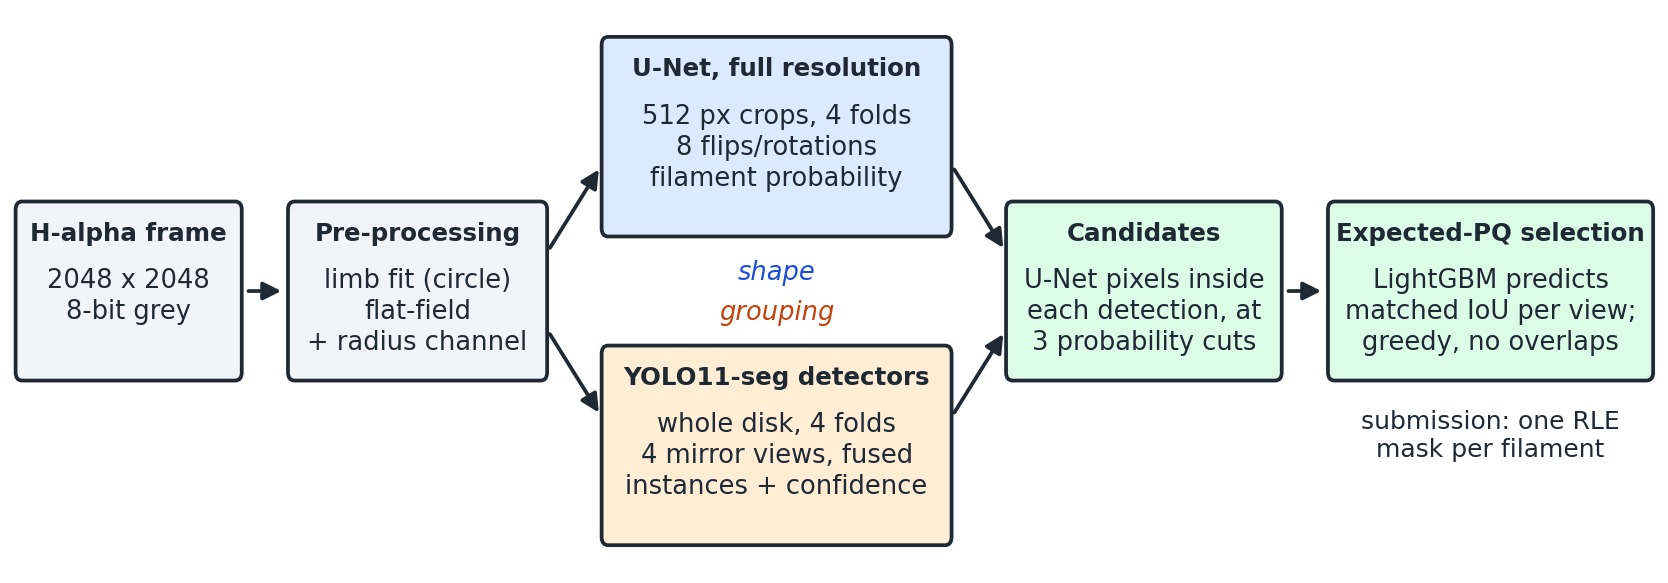
\includegraphics[width=0.86\textwidth]{figures/pipeline.png}
    \caption{The pipeline. The U-Net supplies the shape of filament material, the detectors supply the grouping into instances and a confidence, and the selector decides which candidates are submitted.}
    \label{fig:pipeline}
\end{figure*}

\subsection{Pre-processing}
    Frames are $2048\times2048$ 8-bit images. \textbf{Limb fit.} The Sun is centred and has a nearly constant radius in GONG frames, so we search for the limb within $\pm45$ pixels of the nominal radius: along each of 360 rays the limb is the radius of steepest brightness drop, and a circle is fitted to these points by least squares with outlier rejection (prominences). A brightness threshold is not used because the halo outside the limb is as bright as the disk in some frames. \textbf{Flat-fielding.} The frame is divided by a Gaussian average ($\sigma=48$ pixels) computed only over disk pixels, which removes limb darkening; a value of 1 then means ``as bright as the surrounding quiet Sun'' anywhere on the disk. The networks receive three channels: the raw image, the flat-fielded image, and the distance from the disk centre in solar radii.

\subsection{Shape: a U-Net at full resolution}
    A U-Net \cite{ronneberger2015unet} with an ImageNet-pretrained ResNet-34 encoder \cite{he2016resnet,iakubovskii2019smp} predicts, for every pixel, the probability that it lies inside a drawn filament. It is trained on random $512\times512$ crops at native resolution: 70\,\% of the crops are centred near a drawn filament and 30\,\% are drawn uniformly over the disk. \textbf{Every annotator's drawing is its own training sample}; where annotators disagree the network therefore learns the fraction of them who marked the pixel, and a probability of 0.5 is their majority vote. Augmentations are the eight symmetries of the square, free rotation (probability 0.5), brightness and contrast jitter, and Gaussian blur. The loss is binary cross-entropy plus soft Dice. We train for 12\,000 iterations with batch size 12, AdamW (learning rate $3\times10^{-4}$, weight decay $10^{-4}$), 500 warm-up iterations followed by cosine decay, mixed precision, and keep an exponential moving average of the weights (decay 0.999). No checkpoint is selected on validation data. At inference the frame is covered by $1024$-pixel tiles overlapping by 256 pixels; logits are averaged over the eight symmetries and blended across tiles with a Hann window.

\subsection{Grouping: YOLO11-seg detectors}
    Thresholding the U-Net output and taking connected components is a poor instance segmentation: one filament often appears as several dark fragments, and neighbouring filaments touch. We therefore train YOLO11-seg detectors \cite{yolo11} on the whole disk, rendered as a three-channel image (raw, flat-fielded, contrast-stretched flat-fielded): \detectorList{}. Both start from COCO weights and use mosaic, scale, mirror and free-rotation augmentation; again each annotator's drawing is a separate sample, so the confidence of a detection approaches the fraction of annotators who draw the object. At inference each detector sees the frame and its three mirror images. Detections from all detectors and views are fused: masks with IoU above 0.5 are one object, represented by the most confident mask and scored by the mean confidence over all voters, counting zero for a voter that missed it.

\subsection{Candidates}
    The detector masks are less precise than the U-Net outline (Table~\ref{tab:ablation}), but they say which pixels go together. For each detection, a \emph{candidate} is the set of pixels whose U-Net probability exceeds a cut and that lie inside the detection's mask grown by 6 pixels. We use three cuts (0.35, 0.5, 0.65), i.e.\ a fatter and a thinner version of each object, and describe every candidate by \nFeatures{} features: detector confidence and agreement; whether the detection lies inside a more confident one or contains less confident ones (the same filament is often proposed both whole and in pieces); U-Net probability inside the candidate and in a ring around it; contrast with the surroundings; length, width, solidity and number of fragments; and distance from the disk centre. Our second final entry additionally offers each connected component of the U-Net foreground as a candidate, i.e.\ the U-Net's own grouping; it scores \pqComp{} out-of-fold against \pqAll{} and \pqCompPublic{} on the public leaderboard.

\subsection{Selection by expected Panoptic Quality}\label{sec:selection}
    The metric is $\mathrm{PQ}=\sum_{\mathrm{TP}}\mathrm{IoU}\,/\,(|\mathrm{TP}|+\tfrac12|\mathrm{FP}|+\tfrac12|\mathrm{FN}|)$, pooled over every annotator's view of every frame. Consider one candidate in a frame with $V$ views that matches a drawing in $m$ of them with IoUs summing to $s$. Submitting it adds $s$ to the numerator. In each matching view a false negative (weight $\tfrac12$) becomes a true positive (weight 1), and in each of the other $V-m$ views the candidate is a false positive (weight $\tfrac12$), so the denominator grows by $\tfrac12 V$ whatever $m$ is. Hence submitting the candidate raises PQ if and only if
    \begin{equation}
        v \;=\; \frac{s}{V} \;>\; \frac{\mathrm{PQ}}{2},
    \end{equation}
    where the \emph{value} $v$ is the candidate's matched IoU averaged over views (zero in views where it matches nothing). The value rewards exactly what the metric rewards: being matched at all, being matched tightly, and being drawn by most annotators. We train gradient-boosted regressors (LightGBM \cite{ke2017lightgbm}; five models of 400 trees with 15 leaves, differing in their random subsampling and averaged) to predict $v$ from the candidate's features, using candidates produced by networks that had not seen the frame. Candidates are then visited by decreasing predicted value and accepted while the value exceeds a threshold $\tau$, unless more than 25\,\% of the candidate is already covered by accepted instances; covered pixels are removed, so submitted instances never overlap. The rule predicts $\tau\approx\mathrm{PQ}/2\approx0.22$; cross-validation selects $\tau=\tauChosen{}$. Fitted separately for each annotation group, the best threshold lies between \tauGroupMin{} and \tauGroupMax{}, and using \tauChosen{} instead costs any group at most \tauGroupLoss{} PQ, so the choice does not depend on who annotated a frame.

\subsection{Splits and training protocol}
    The \nFrames{} training frames (\nViews{} views, \nDrawings{} drawings) are split into four folds \emph{by frame}, stratified by the number of annotators, so all drawings of a frame stay together. For each fold a U-Net and the detectors are trained on the other three folds and applied to the held-out fold and to the test set. The selector is trained on the held-out candidates of all folds and is itself cross-fitted over frames when it is evaluated. For the submission the U-Net probabilities and the detections of the four folds are averaged and fused, respectively. The test images were used for inference only, and no annotation other than the competition's training file was used at any point.

%                                      %
%              EVALUATION              %
%                                      %
\section{Evaluation}\label{sec:evaluation}

\subsection{Strategy}
    All validation numbers are out-of-fold: every training frame is predicted by networks and by a selector fitted without it. We reimplemented the organizers' scorer on run-length masks (it reproduces the reference on our unit tests) and report PQ, detection quality (DQ) and segmentation quality (SQ) with 95\,\% bootstrap intervals obtained by resampling frames 2\,000 times.

\begin{table}[t]
    \caption{Out-of-fold results on the \nFrames{} training frames, with 95\,\% bootstrap intervals for PQ.}
    \label{tab:main}
    \small
        \begin{tabular}{lrccc}
        \toprule
        Frames & $n$ & PQ [95\,\% interval] & DQ & SQ \\
        \midrule
        All & 532 & 0.450 [0.440, 0.460] & 0.659 & 0.683 \\
        1 annotator & 309 & 0.456 [0.443, 0.470] & 0.663 & 0.688 \\
        2 annotators & 109 & 0.455 [0.432, 0.477] & 0.667 & 0.682 \\
        3 annotators & 114 & 0.440 [0.422, 0.458] & 0.650 & 0.677 \\
        \midrule
        Annotator vs.\ annotators & 223 & 0.344 [0.325, 0.363] & 0.542 & 0.634 \\
        \bottomrule
    \end{tabular}

\end{table}

\begin{table}[t]
    \caption{What each component contributes (out-of-fold PQ).}
    \label{tab:ablation}
    \small
        \begin{tabular}{lc}
        \toprule
        Variant & PQ \\
        \midrule
        U-Net connected components (no detector) & 0.416 \\
        Detector masks (no U-Net) & 0.416 \\
        U-Net pixels in detections, one detector, one view & 0.441 \\
        \quad + second detector and mirror views & 0.447 \\
        \quad + three probability cuts and learned selector (full) & 0.453 \\
        Oracle selection of the same candidates & 0.545 \\
        \bottomrule
    \end{tabular}

\end{table}

\begin{table}[t]
    \caption{Out-of-fold PQ by observing site of the GONG network.}
    \label{tab:sites}
    \small
        \begin{tabular}{lrc}
        \toprule
        GONG site & $n$ & PQ [95\,\% interval] \\
        \midrule
        Big Bear & 93 & 0.447 [0.424, 0.468] \\
        Cerro Tololo & 97 & 0.455 [0.432, 0.477] \\
        Learmonth & 101 & 0.442 [0.419, 0.465] \\
        Mauna Loa & 89 & 0.438 [0.413, 0.462] \\
        El Teide & 80 & 0.458 [0.433, 0.482] \\
        Udaipur & 72 & 0.464 [0.437, 0.496] \\
        \bottomrule
    \end{tabular}

\end{table}

\subsection{Results}
    Table~\ref{tab:main} gives the main result, PQ~\pqAll{} [\pqAllLow{}, \pqAllHigh{}], against \pqHuman{} for one annotator scored against the others. Frames drawn by three annotators score slightly lower than frames drawn by one, although the intervals overlap: a filament that only one of three annotators drew is a false positive in the two other views. On the \thirdFrames{} frames drawn by three annotators, one annotator predicts the drawing of another with PQ~\thirdOne{}, the filaments on which two annotators agree predict the third annotator's drawing with PQ~\thirdTwo{}, and the method predicts it with PQ~\thirdMethod{}: the method is a better predictor of what an annotator draws than other annotators are. The public leaderboard, which uses about half of the test frames, gives \pqPublic{}. The score is stable across the six observing sites (Table~\ref{tab:sites}), whose seeing and image quality differ. Table~\ref{tab:ablation} isolates the components. \ablationText{} Neither network is sufficient alone: the detector masks lose \ablationShapeGain{} PQ against the same detections filled with U-Net pixels, and the U-Net components lack the grouping. The metric is very sensitive to the outline: shrinking every submitted instance by one pixel lowers PQ by \outlineMinus{}, and growing it by one pixel lowers it by \outlinePlus{}, so the U-Net boundary sits at the optimum.

    Fig.~\ref{fig:dist} shows the distributions requested by the organizers. Among overlapping pairs the IoU has its mode above the matching threshold but a sizeable mass between 0.3 and 0.5: pairs that agree on the object but not closely enough on its extent. Most drawings overlap exactly one prediction and most predictions exactly one drawing; one-to-many relations are rare, which shows that fragmentation is largely resolved by the detector grouping. Fig.~\ref{fig:examples} shows the submitted instances on a test frame and typical held-out predictions together with the three annotators' drawings.

\begin{figure}[t]
    \centering
    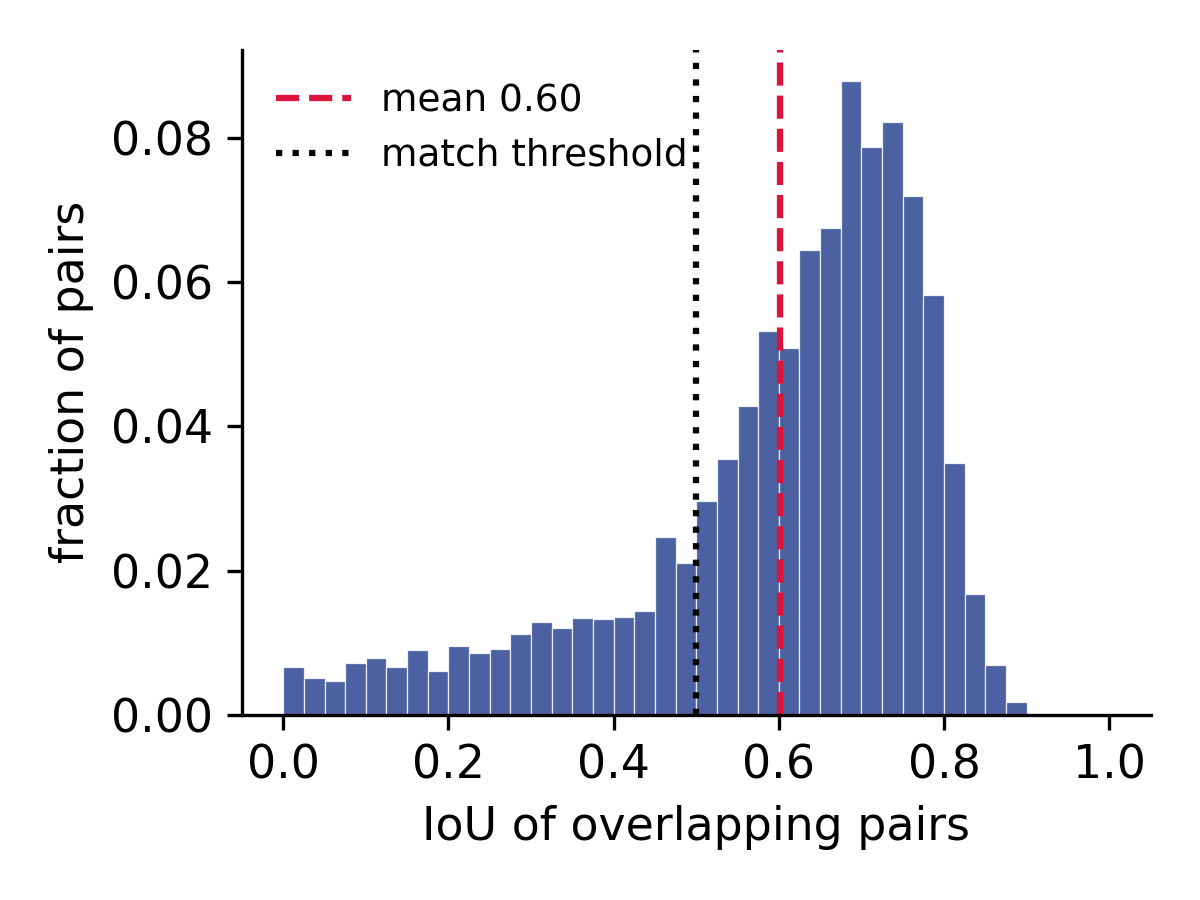
\includegraphics[width=0.49\columnwidth]{figures/iou_distribution.png}\hfill
    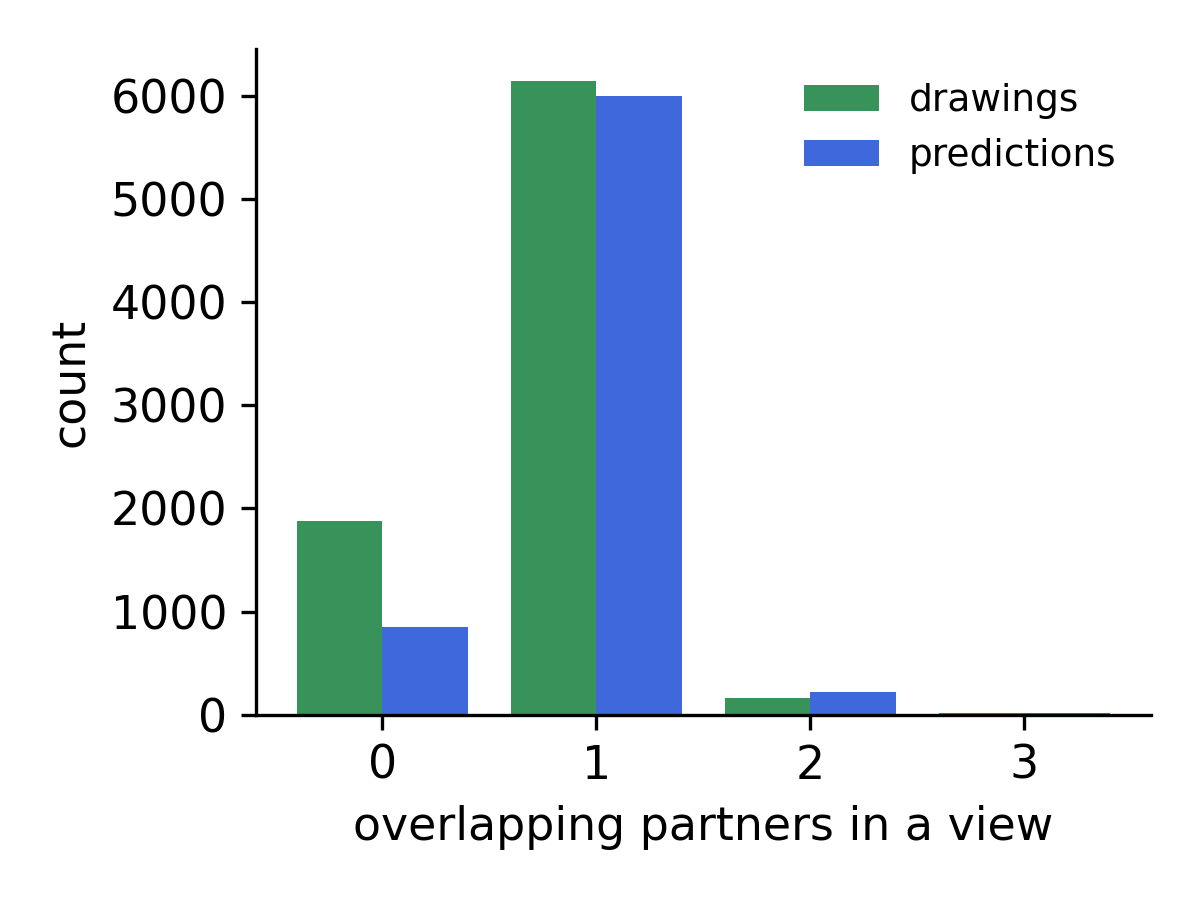
\includegraphics[width=0.49\columnwidth]{figures/relations.png}
    \caption{Out-of-fold predictions against every annotator view. Left: IoU of all overlapping (drawing, prediction) pairs. Right: number of predictions each drawing overlaps, and number of drawings each prediction overlaps (0 = missed or spurious, 1 = one-to-one).}
    \label{fig:dist}
\end{figure}

\begin{figure*}[t]
    \centering
    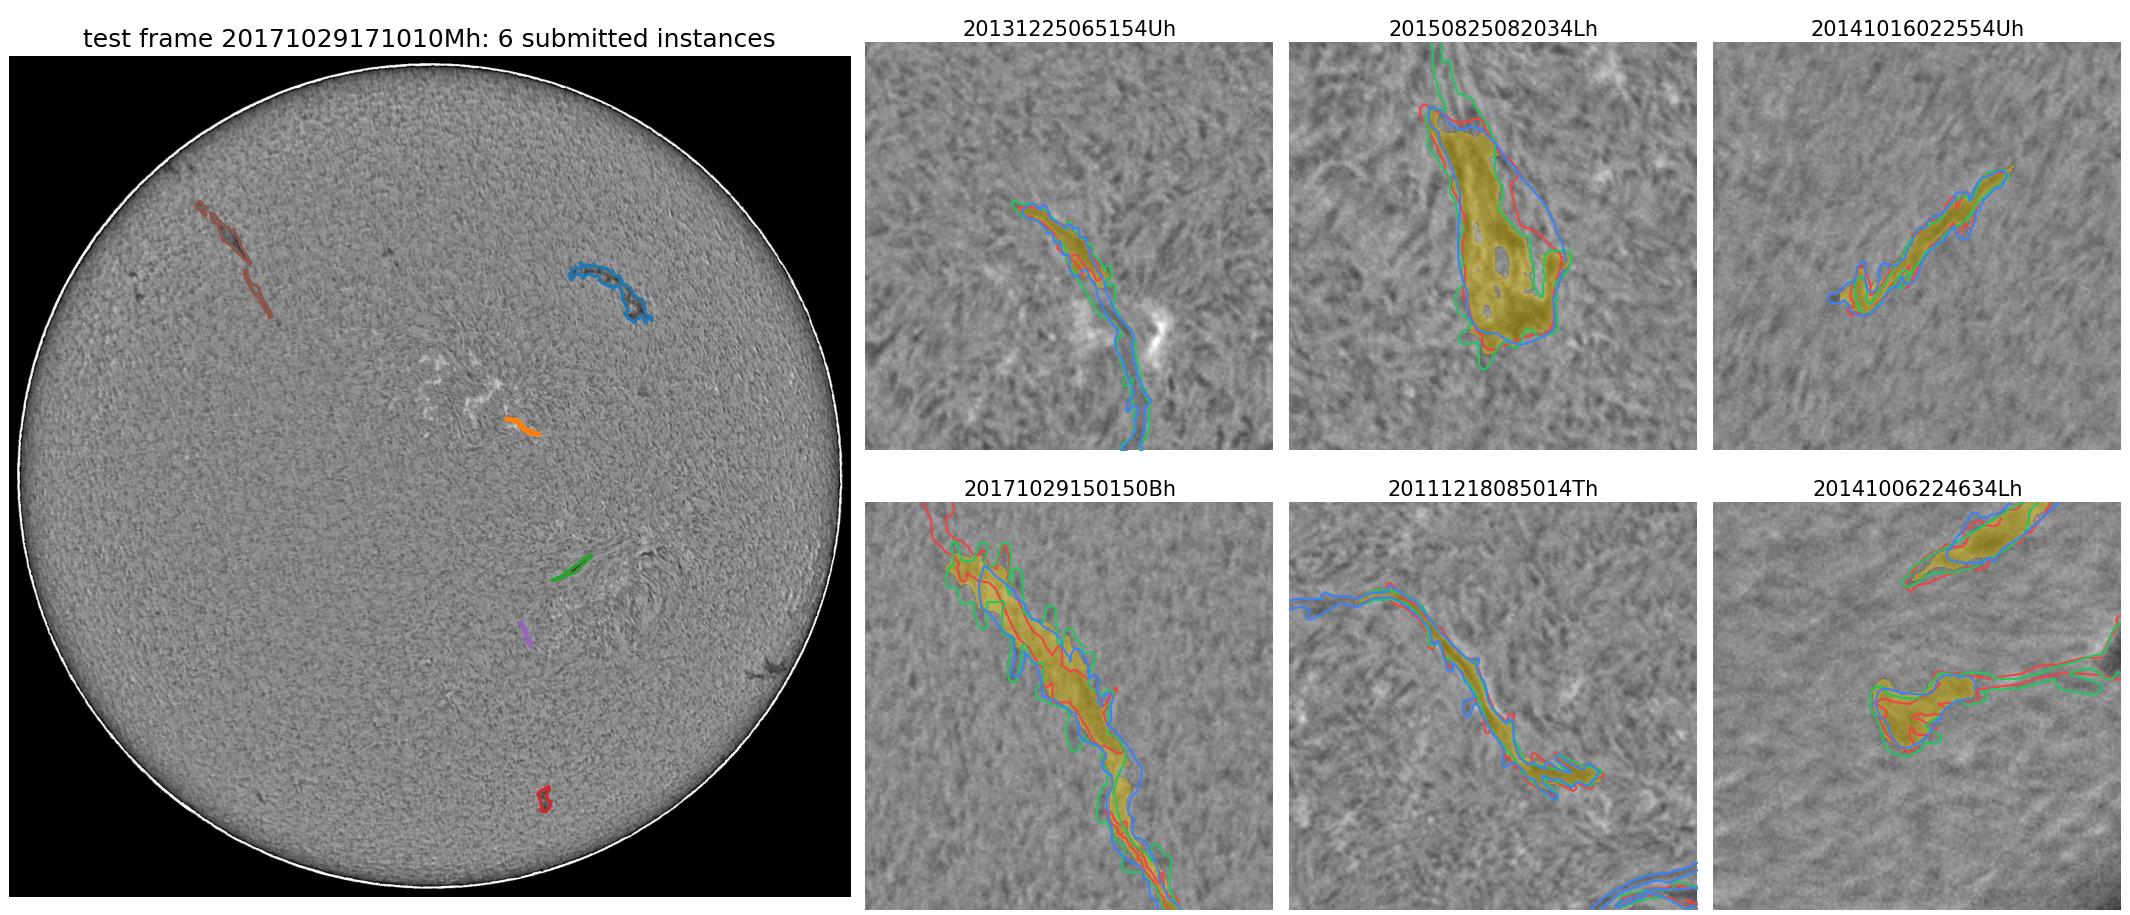
\includegraphics[width=\textwidth]{figures/examples.png}
    \caption{Left: a test frame (flat-fielded) with the submitted instances, one colour each. Right: out-of-fold predictions (yellow) on held-out training frames drawn by three annotators (red, green and blue outlines). The annotators agree on prominent filaments and differ on faint ones and on where a filament ends.}
    \label{fig:examples}
\end{figure*}

\subsection{Strengths, weaknesses and next steps}
    \textbf{Strengths.} The outlines come from a full-resolution network and are tighter than the annotators' mutual agreement (SQ~\sqAll{} against \sqHuman{}). The selection rule is derived from the metric rather than tuned by hand, and the whole pipeline is validated out-of-fold, including the selector. Inference needs only the test images.

    \textbf{Weaknesses.} An oracle that knows each candidate's true value would reach PQ~\pqOracle{} with the same candidates, so most of the remaining loss is in deciding \emph{which} candidates an annotator would draw. Much of that decision is the annotators' own disagreement, which no predictor can remove, and the selector adds little to the detector's confidence (Table~\ref{tab:ablation}). \missedShare{} of the drawings have no candidate with IoU above 0.5, mostly small or faint filaments and filaments whose extent the annotators draw differently. Resolution is not the cause: adding a third detector at the native $2048^2$ pixels raises the out-of-fold PQ only to \threeDetPQ{} (difference \threeDetGain{}, 95\,\% interval \threeDetLow{} to \threeDetHigh{}), which does not exclude zero, so it was not adopted. Long filaments that annotators split differently cannot be matched in every view by one non-overlapping prediction. The leaderboard score is about 0.87 times the out-of-fold score, for every submission we made and for other participants who report both numbers. On the training data the score varies far more between the \nGroups{} annotation groups (PQ \groupMin{} to \groupMax{}) than between observing sites (\siteMin{} to \siteMax{}), so the factor is consistent with test frames drawn by different annotators rather than with over-fitting.

    \textbf{Next steps.} A refinement network that redraws each instance given its group, trained on the annotators' polygons; using consecutive GONG frames, since filaments persist for days; and predicting a distribution over groupings so that the selection can trade a whole filament against its pieces explicitly.

\subsection{Implementation and reproducibility}
    The code, the trained weights and a notebook that rebuilds the submitted file without retraining are available at \url{REPOSITORY-URL}. Training one fold takes 1.3 hours for the U-Net and 5.5 and 1.6 hours for the two detectors on one Tesla T4; the selector is fitted on a CPU in minutes. Inference on the 180 test frames takes \inferenceMinutes{} minutes on \inferenceGpu{}; rebuilt this way from the released weights, the submission matches the submitted file in all 1\,164 instances (pixel-level agreement PQ 0.9998, against 1 for identical files). Software: PyTorch 2.11, segmentation\_models\_pytorch 0.6, Ultralytics 8.4 and LightGBM 4.7; exact versions are pinned in \texttt{requirements.txt}. The fold assignment is a deterministic function of the annotation file; training is not bit-reproducible (random crops, GPU arithmetic), which is why the weights are released.

%                                      %
%            ACKNOWLEDGMENT            %
%                                      %
\section{Acknowledgment}\label{sec:acknowledgment}
    % Do not change
    The organization of the Filament Segmentation Challenge 2026 is partially supported by the U.S. National Science Foundation (NSF) under Grant No. 2209912 and 2433781, directorate for Computer and Information Science and Engineering (CSE), and Office of Advanced Cyberinfrastructure (OAC), and Grant No. 2511630, AST Division Of Astronomical Sciences and MPS Directorate for Mathematical and Physical Sciences.

    The Filament Segmentation Challenge 2026 is sponsored by the U.S. National Science Foundation (NSF) National Solar Observatory (NSO).

    This work utilizes GONG data obtained by the NSO Integrated Synoptic Program, managed by the National Solar Observatory, which is operated by the Association of Universities for Research in Astronomy (AURA), Inc. under a cooperative agreement with the National Science Foundation and with contribution from the National Oceanic and Atmospheric Administration. The GONG network of instruments is hosted by the Big Bear Solar Observatory, High Altitude Observatory, Learmonth Solar Observatory, Udaipur Solar Observatory, Instituto de Astrofísica de Canarias, and Cerro Tololo Interamerican Observatory.

\bibliographystyle{ACM-Reference-Format}
\bibliography{main}

\end{document}
